\documentclass[11pt,letterpaper]{article}

% include figures
\usepackage{graphicx}
\usepackage{caption,subcaption}
% get nice colors
\usepackage{xcolor}

% change default font to Palatino (looks nicer!)
\usepackage[latin1]{inputenc}
\usepackage{mathpazo}
\usepackage[T1]{fontenc}
% load some useful math symbols/fonts
\usepackage{latexsym,amsfonts,amsmath,amssymb,wasysym}
% be able to insert code
\usepackage{listings}

% comfort package to easily set margins
\usepackage[top=1in, bottom=1in, left=1in, right=1in]{geometry}

% spacing after a paragraph
\setlength{\parskip}{.15cm}
% indentation at the top of a new paragraph
\setlength{\parindent}{0.0cm}
% make units not slanted in math mode
\newcommand{\unit}[1]{\ensuremath{\, \mathrm{#1}}}

\begin{document}

\begin{center}
\Large
Ay190 -- Worksheet 15\\
Daniel DeFelippis\\
Date: \today
\end{center}

%%
%%
%% I worked with Scott Barenfeld
%%
%% All python code can be found in the ws15 directory in my repository
%%
%%

\section*{1D SPH Code}

\section{}

The program we are running here does "Smoothed Particle Hydrodynamics." This method
centers on using a smoothing kernel to deal with a large amount of gas particles.
The field of particles (really the field of a property of the particles like density)
is convolved with this smoothing kernel:
$$ F_{smooth}(r) = \int F(r) W(r-r',h)dr' $$ 
where $W$ is the smoothing kernel, and $h$ is the characteristic length scale of the 
smoothing. This kernel will be equal to 0 for values of $r'$ for, in this case, 
particles farther than 2 scale lengths away from a given particle. Particles between
0 and 1 scale lengths away, and between 1 and 2 scale lengths away, have two different values
for the smoothing kernel, as shown by the code below.
\lstinputlisting[language=Python, firstline=23, lastline=31]{ws15.py}

Here, since we have discrete particles, the integral above is really a sum:
$$ F_s(r) \approx \sum\limits_j \frac{m_j}{\rho_j}F_j W(r-r_j,h) $$
where $m$ and $\rho$ are the mass and density at the location of particle $j$. 

Now, for computing any fields, we need to know how many particles are nearer than twice
the scale length from a given particle, which the function "neighbor\_search\_1D" does.
Given that, the functions "smoothing\_kernel" (code copied above) and
"dsmoothing\_kernel\_rij" compute the kernel and the grad of the kernel, which we
will need for computing other things. 

For example, the smoothed density at the location of particle $i$ is given by 
$$\rho_i \approx \sum\limits_j \frac{m_j}W(r-r_j,h)$$.
which we can calculate using the functions listed above, since we have inital values
of densities from which we can get masses. THe function "get\_density" does this.

One other variable we need to calculate is the artificial viscosity, which increases 
the entropy of the system during shocks. Each particle will have an artificial 
viscosity with each of its neighbors, and the function "get\_artificial\_viscosity" 
does this. 

There are two main equations which this system uses to evolve (the other variables 
evolve according to those two equations): the momentum equaition and energy equations:
\begin{align*}
\frac{dv_i}{dt} &= -\sum\limits_{j=1}^n m_j \left(\frac{P_i}{\rho_i^2} + \frac{P_j}{\rho_j^2} + \prod\limits_{ij} \right) \nabla W_{ij}(h) \\
\frac{d\epsilon_i}{dt} &= \frac{1}{2}\sum\limits_{j=1}^n m_j \left(\frac{P_i}{\rho_i^2} + \frac{P_j}{\rho_j^2} + \prod\limits_{ij} \right) v_{ij} \nabla W_{ij}(h) 
\end{align*}
where $\prod\limits_{ij}$ is the artificial viscosity term and $P$ is pressure (calculated
from equation of state using density and energy). The function "get\_accels" uses a nested
for loop to calculate $\frac{dv_i}{dt}$ for all particles $i$:
\lstinputlisting[language=Python, firstline=113, lastline=116]{ws15.py}
and the function "get\_energyRHS" uses the same process to calculate $\frac{d\epsilon_i}{dt}$
for all particles $i$:
\lstinputlisting[language=Python, firstline=131, lastline=134]{ws15.py}

The actual program first sets the initial densities, energies, and velocities. The densities
are different for the left and right side, as are the energies, and the velocities are all 0.
From these, it calculates the pressures and speeds of sound. Then it runs the neighbor search
function so it can calculate the smoothed density. After initializing the timestep, the
program finally starts evolving the system. 

For each iteration, it calculates artificial 
viscosities, then accelerations (RHS of momentum equations). The accelerations are
used to update the velocities and half step velocities, and then the positions. It also
calculates the new RHS of the energy equation, which is used to update the energy. 

After all this, it updates all of the variables initialized above, updates the plot, and
increases the time (i.e. goes to the next iteration which is dt later than the current one).

Plots of every 20 iterations are shown in figures~\ref{fig:it1and20} to ~\ref{fig:it160} 
below, including the first iteration. (i.e., 1, 20, 40, ... , 160).

\begin{figure}[bth]
\centering
\begin{subfigure}{.5\textwidth}
  \centering
  \includegraphics[width=.95\linewidth]{out_0001.pdf}
  \caption*{Density profile: Iteration 1}
  \label{fig:sub1}
\end{subfigure}%
\begin{subfigure}{.5\textwidth}
  \centering
  \includegraphics[width=.95\linewidth]{out_0020.pdf}
  \caption*{Iteration 20}
  \label{fig:sub2}
\end{subfigure}
\caption{}
\label{fig:it1and20}
\end{figure}

\begin{figure}[bth]
\centering
\begin{subfigure}{.5\textwidth}
  \centering
  \includegraphics[width=.95\linewidth]{out_0040.pdf}
  \caption*{Iteration 40}
  \label{fig:sub3}
\end{subfigure}%
\begin{subfigure}{.5\textwidth}
  \centering
  \includegraphics[width=.95\linewidth]{out_0060.pdf}
  \caption*{Iteration 60}
  \label{fig:sub4}
\end{subfigure}
\caption{}
\label{fig:it40and60}
\end{figure}

\begin{figure}[bth]
\centering
\begin{subfigure}{.5\textwidth}
  \centering
  \includegraphics[width=.95\linewidth]{out_0080.pdf}
  \caption*{Iteration 80}
  \label{fig:sub5}
\end{subfigure}%
\begin{subfigure}{.5\textwidth}
  \centering
  \includegraphics[width=.95\linewidth]{out_0100.pdf}
  \caption*{Iteration 100}
  \label{fig:sub6}
\end{subfigure}
\caption{}
\label{fig:it80and100}
\end{figure}

\begin{figure}[bth]
\centering
\begin{subfigure}{.5\textwidth}
  \centering
  \includegraphics[width=.95\linewidth]{out_0120.pdf}
  \caption*{Iteration 120}
  \label{fig:sub5}
\end{subfigure}%
\begin{subfigure}{.5\textwidth}
  \centering
  \includegraphics[width=.95\linewidth]{out_0140.pdf}
  \caption*{Iteration 140}
  \label{fig:sub6}
\end{subfigure}
\caption{}
\label{fig:it120and140}
\end{figure}

\begin{figure}[bth]
\centering
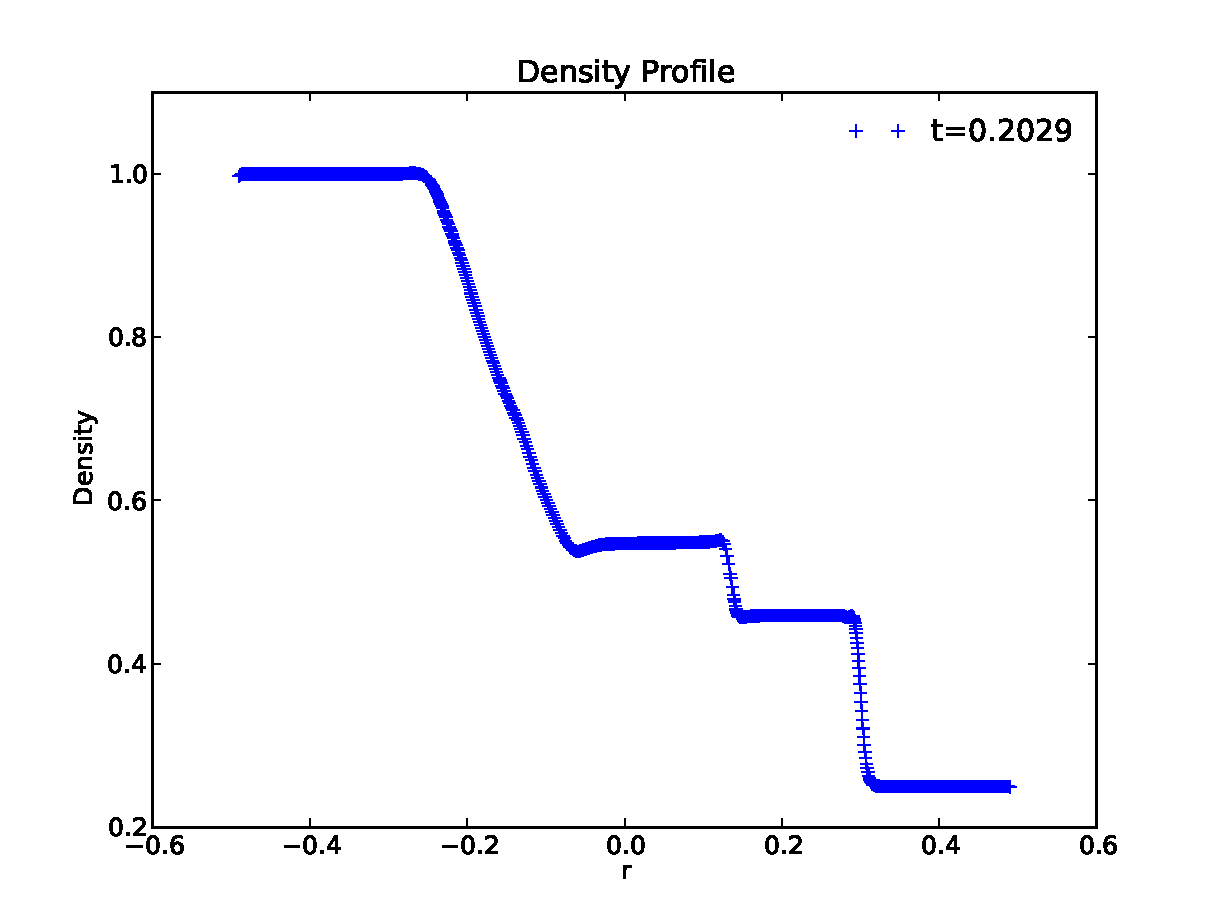
\includegraphics[width=0.5\textwidth]{out_0160.pdf}
\caption{Iteration 160}
\label{fig:it160}
\end{figure}

We see the expected zones: the first and fifth are constant with the initial densities
as the value, and there is a rarefaction zone as well as clear contact and shock 
close-to-vertical lines.


\section{}

We now use the Riemann solver written in Fortran. We can plot the density profile of 
the Riemann solver at $t=0.2$ (after editing the desired time and position values) 
with the density profile of the SPH code at the same time,
as well as other variables which the program calculates: velocity and pressure. 
As expected, the plots in figures~\ref{fig:density}, \ref{fig:velocity}, 
and \ref{fig:pressure} demonstrate that the SPH solver matches the exact solver 
very well. There are notable differences though. As shown in the density profile 
(figure~\ref{fig:density}), the corners of the SPH solution look "overcurved" 
compared to the sharp corners of the exact solution. Additionally, 
what are supposed to be vertical lines at around $x=0.15$
and $x=0.3$ are slanted in the SPH solution. In the velocity profile 
(figure~\ref{fig:velocity}), there is a small bump at the end of the rarefaction zone
that is present in the SPH solution but not the exact solution. 
In the pressure profile (figure~\ref{fig:pressure}), there is what appears to be 
an instability in the SPH solution at around $x=0.15$, which is the location of the
contact. It isn't in the exact solution, which 
suggests that the SPH solver isn't the best at calculating the pressures at the
boundaries of the zones.

\begin{figure}[bth]
\centering
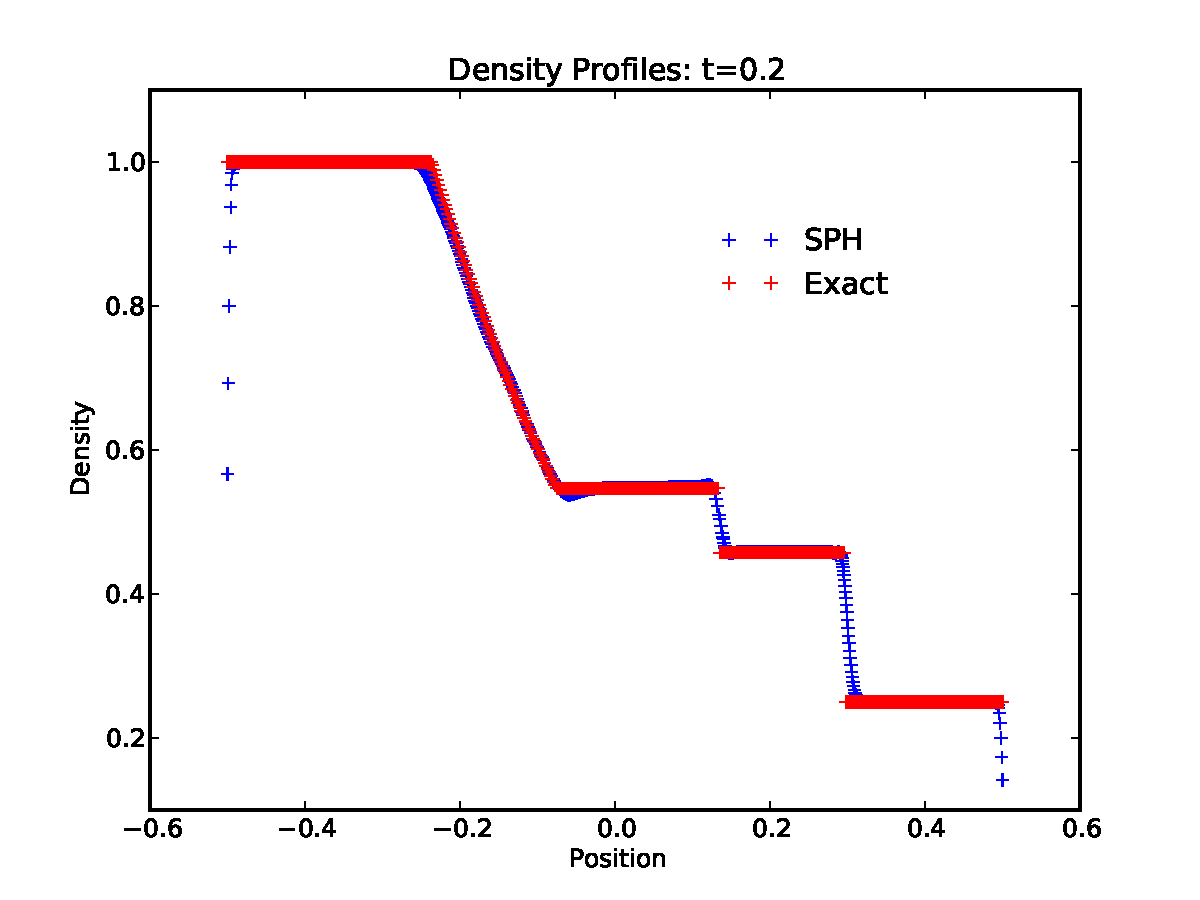
\includegraphics[width=0.75\textwidth]{density.pdf}
\caption{Density profiles of SPH and exact Riemann solver at $t=0.2$.}
\label{fig:density}
\end{figure}

\begin{figure}[bth]
\centering
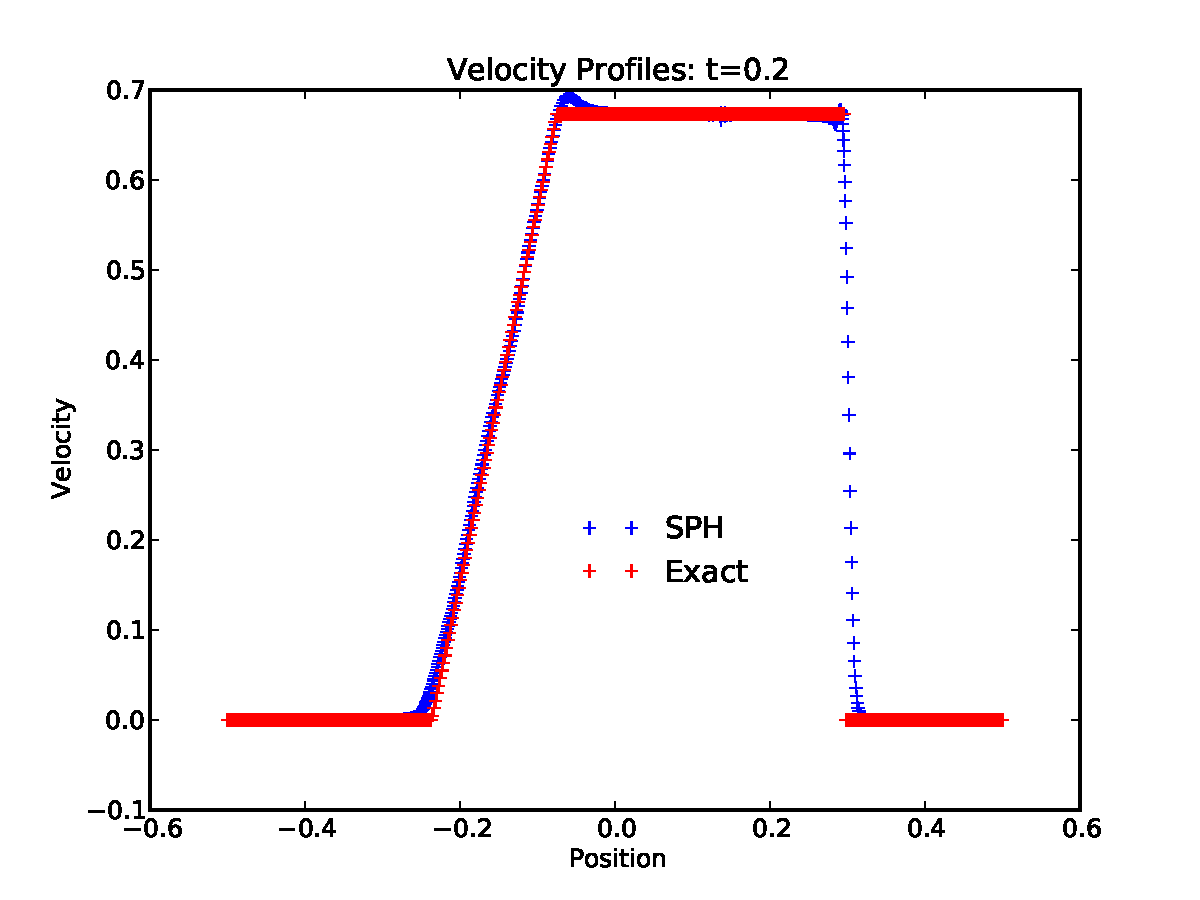
\includegraphics[width=0.75\textwidth]{velocity.pdf}
\caption{Velocity profiles of SPH and exact Riemann solver at $t=0.2$.}
\label{fig:velocity}
\end{figure}

\begin{figure}[bth]
\centering
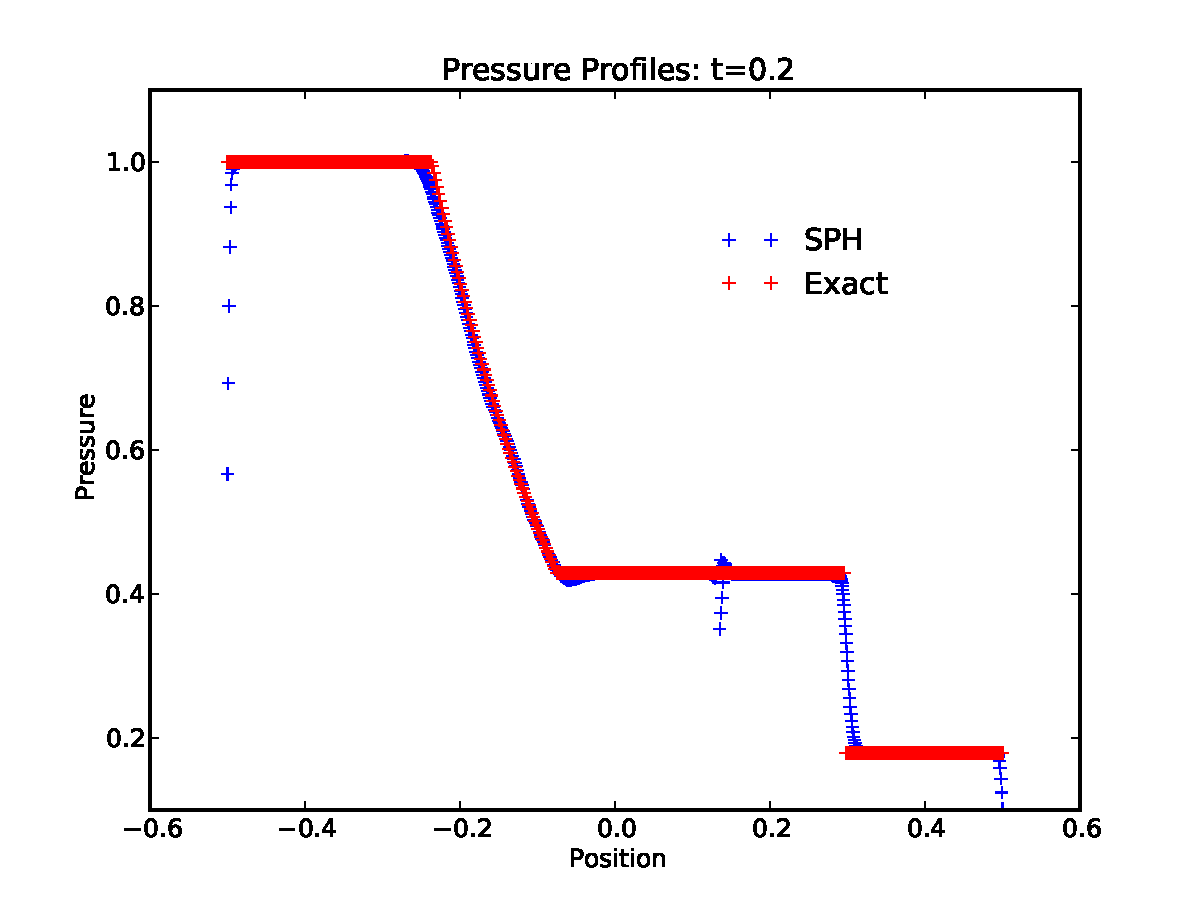
\includegraphics[width=0.75\textwidth]{pressure.pdf}
\caption{Pressure profiles of SPH and exact Riemann solver at $t=0.2$.}
\label{fig:pressure}
\end{figure}

\end{document}
